\documentclass[preprint,12pt]{elsarticle}
%\documentclass[review]{elsarticle}
\usepackage{lineno,hyperref}
\usepackage{booktabs}
\usepackage[english]{babel}
\usepackage[utf8]{inputenc}
\usepackage{amsfonts}
\usepackage{graphicx}
%\usepackage[colorinlistoftodos]{todonotes}
\usepackage{amssymb,amsmath}
\usepackage{float}
\usepackage{ragged2e}
\usepackage{array}
\usepackage{multirow}
\usepackage{adjustbox}
\usepackage{multicol}
\usepackage{mwe}
%\usepackage{caption}
\usepackage[justification=centering]{caption}

\usepackage{algorithm}
%\usepackage{algorithm2e}
%\usepackage{algorithmicx}
\usepackage{algpseudocode}

\usepackage{multirow}
\usepackage{mathtools}
\usepackage{color}
\usepackage{soul}
\usepackage{comment}
\usepackage{lscape}
\usepackage{setspace}
\usepackage{tikz}
\usetikzlibrary{shapes.geometric, arrows.meta, positioning, fit, backgrounds}
\doublespacing

\algnewcommand\algorithmicforeach{\textbf{for each}}
\algdef{S}[FOR]{ForEach}[1]{\algorithmicforeach\ #1\ \algorithmicdo}

\newcommand\tab[1][0.73cm]{\hspace*{#1}}

\def\checkmark{\tikz\fill[scale=0.3](0,.35) -- (.25,0) -- (1,.7) -- (.25,.15) -- cycle;}

\usepackage{array}
\newcolumntype{L}[1]{>{\raggedright\let\newline\\\arraybackslash\hspace{0pt}}m{#1}}
\newcolumntype{C}[1]{>{\centering\let\newline\\\arraybackslash\hspace{0pt}}m{#1}}
\newcolumntype{R}[1]{>{\raggedleft\let\newline\\\arraybackslash\hspace{0pt}}m{#1}}
\newcolumntype{P}[1]{>{\centering\arraybackslash}p{#1}}
\newcolumntype{M}[1]{>{\centering\arraybackslash}m{#1}}

\def\arrvline{\hfil\kern\arraycolsep\vline\kern-\arraycolsep\hfilneg}

\modulolinenumbers[5]

\journal{Elsevier}

%% `Elsevier LaTeX' style
\bibliographystyle{elsarticle-num}

%%%%%%%%%%%%%%%%%%%%%%%

\begin{document}

\begin{frontmatter}

\title{Smart Classroom Analytics: A Computer Vision Based System for Automated Attendance, Student Engagement Analysis, and Classroom Activity Monitoring}

\author[1]{Nikhil Kumar\corref{cor1}}
\ead{nikhil23bcs45@iiitkottayam.ac.in}

\author[1]{Gaurav Kumar}
\ead{gaurav23bcs114@iiitkottayam.ac.in}

\author[1]{Adarsh Dubey}
\ead{adarsh23bcs117@iiitkottayam.ac.in}

\author[1]{Ajeet Kumar}
\ead{ajeet23bcs177@iiitkottayam.ac.in}

\cortext[cor1]{Corresponding author}

\address[1]{Department of Computer Science and Engineering,
IIIT Kottayam, Kerala, India}


\begin{abstract}
Manual attendance recording and passive classroom monitoring are among the most persistent inefficiencies in modern educational practice. Roll calls consume lecture time, paper-based sign-ins enable proxy attendance, and unaided observation of engagement across large cohorts is both unreliable and unscalable. This paper presents a Smart Classroom Analytics system that addresses these limitations through a unified, real-time computer vision pipeline integrating three synergistic modules. The attendance module employs a ResNet-50 backbone trained with an ArcFace loss to extract discriminative identity embeddings, enabling simultaneous recognition of multiple students from unconstrained classroom video under occlusion, illumination variation, and non-frontal head poses. The engagement analysis module fuses Facial Action Unit (AU) vectors extracted via OpenFace 2.0 with head pose angles and eye-gaze direction, feeding a tri-class classifier that labels each student as \textit{engaged}, \textit{partially engaged}, or \textit{disengaged} at 15\,fps. The classroom activity monitoring module leverages a lightweight YOLOv8-nano backbone to detect off-task behaviors including mobile phone usage, sleeping, and note-taking. All three modules share a common video ingestion front-end and operate on standard commodity hardware without requiring modifications to the physical classroom environment. Experiments on the DAiSEE and EngageNet benchmark datasets, supplemented by real classroom recordings, demonstrate attendance recognition accuracy of 97.4\%, engagement classification F1-score of 0.91 (three-class), and activity detection mAP of 88.6\%, with end-to-end latency below 67\,ms per frame. These results establish a new state-of-the-art for unified, multi-task classroom analytics and confirm the practical deployability of the proposed system.
\end{abstract}

\begin{keyword}
Smart Classroom \sep Face Recognition \sep Student Engagement \sep Attendance Automation \sep Computer Vision \sep Deep Learning \sep Behavioral Analysis \sep ArcFace \sep YOLOv8 \sep OpenFace
\end{keyword}

\end{frontmatter}

\linenumbers

%% ============================================================
\section{Introduction}
%% ============================================================

Modern educational institutions are under increasing pressure to improve the quality and efficiency of classroom management while simultaneously fostering deeper student learning. Two persistent operational challenges underlie this pressure: the manual recording of student attendance and the lack of objective, scalable mechanisms for monitoring student engagement during lectures. Both tasks are currently performed through labor-intensive, subjective, and error-prone methods. Roll calls consume valuable lecture time, paper-based sign-in sheets are susceptible to proxy attendance, and the unaided human observation of engagement cues across a large class is fundamentally unreliable. The convergence of affordable high-resolution cameras, advances in deep learning, and the growing adoption of smart classroom infrastructure creates a timely opportunity to address these challenges through a unified, automated computer vision (CV) pipeline.

Automated attendance systems built on biometric recognition offer a natural starting point. Among available biometric modalities --- fingerprint, iris, and voice recognition --- face recognition is uniquely suited to the classroom context because it is contactless, non-intrusive, and requires no active cooperation from the student \cite{attendance_android}. Early systems relied on classical computer vision techniques such as Eigenfaces, Local Binary Pattern Histograms (LBPH), and Viola-Jones detectors; however, these approaches degrade significantly under real-world classroom conditions that include partial occlusion, variable illumination, non-frontal head poses, and simultaneous multi-face scenes. The emergence of deep convolutional neural networks (CNNs), and in particular residual architectures such as ResNet-50 \cite{resnet}, has transformed face recognition by learning highly discriminative identity embeddings that are robust to these sources of variation. Ensemble strategies combining multiple deep models have further improved recognition accuracy in unconstrained settings, demonstrating consistent gains over individual architectures \cite{ensemble_ieee}. More recently, margin-based loss functions such as ArcFace \cite{arcface} have pushed recognition accuracy on large-scale benchmarks to levels approaching human performance by introducing an additive angular margin penalty that maximally separates inter-class boundaries in the hyperspherical embedding space.

Beyond attendance, there is growing recognition in the education research community that monitoring student engagement is equally, if not more, important for improving learning outcomes. Engagement is a multi-dimensional construct encompassing behavioral, emotional, and cognitive dimensions, and its decline --- manifesting as distraction, drowsiness, or disengagement --- is a leading predictor of poor academic performance and dropout \cite{engagement_springer}. Detecting engagement from visual cues is a well-established research direction: head pose, gaze direction, facial expressions, and facial action units (AUs) have all been shown to correlate with self-reported and instructor-assessed engagement levels \cite{openface}. The challenge lies in moving beyond single-cue systems to models that jointly exploit facial and behavioral features in a computationally efficient manner suitable for real-time classroom deployment \cite{lit_pose_attention_2025, lit_engagement_multimodal_2025}.

The scope of smart classroom analytics extends further still to encompass the monitoring of broad classroom activity patterns --- including the detection of mobile phone usage, sleeping, note-taking, and group discussion behaviors --- which collectively inform pedagogical decisions and institutional policy. Several recent systems have demonstrated the feasibility of integrating attendance and behavioral monitoring within a single pipeline, exploiting IoT-enabled camera networks and AI inference at the edge \cite{disengagement_ieee, robotic_iot, lit_edge_inference_2025}. However, existing work largely addresses these three tasks --- attendance, engagement, and activity monitoring --- in isolation, and integrated systems that jointly solve all three in a unified architectural framework remain scarce \cite{lit_unified_pipeline_2025}.

This paper proposes a Smart Classroom Analytics system that integrates three synergistic computer vision modules into a single, real-time pipeline: (i) an automated attendance module based on ResNet-50 with ArcFace loss capable of identifying multiple students simultaneously from classroom video streams; (ii) a student engagement analysis module that fuses facial action units extracted via OpenFace 2.0 with behavioral cues such as head pose and eye gaze to classify engagement into three levels --- engaged, partially engaged, and disengaged; and (iii) a classroom activity monitoring module that detects common off-task behaviors using a YOLOv8-nano object and pose detection backbone. The system is designed to operate on standard classroom hardware without requiring modifications to the physical environment, and it produces structured analytical reports that can directly inform instructor interventions.

The salient contributions of this paper are as follows:
\begin{enumerate}
    \item A unified deep learning pipeline that simultaneously performs face recognition-based attendance, multi-level student engagement classification, and classroom activity monitoring from a single video input stream, eliminating the need for separate, disjointed systems.
    \item A multi-feature fusion strategy for engagement detection that jointly models facial action units, head pose, and gaze direction --- demonstrated via ablation to outperform each single-modality baseline individually --- enabling fine-grained tri-class engagement labeling at real-time throughput.
    \item An ArcFace-augmented ResNet-50 attendance module that achieves 97.4\% recognition accuracy under unconstrained classroom conditions including occlusion and multi-face simultaneous recognition, supported by a theoretical analysis of the hyperspherical margin geometry that explains why ArcFace outperforms softmax-based training in the open-set gallery matching scenario.
    \item An end-to-end evaluation on publicly available benchmark datasets and real classroom recordings that benchmarks the proposed system against recent state-of-the-art methods across all three tasks, providing a comprehensive assessment of accuracy, F1-score, and real-time throughput.
\end{enumerate}

The rest of this paper is organized as follows. Section~\ref{section2} surveys related work on face recognition-based attendance systems, student engagement detection, and classroom activity monitoring, identifying key limitations of existing approaches. Section~\ref{section3} describes the proposed system architecture and each module in detail, including novelty analysis and theoretical justification. Section~4 presents the datasets used, the experimental setup, and a comparative analysis of results. Section~5 concludes the paper and outlines directions for future research.

%% ============================================================
\section{Literature Survey} \label{section2}
%% ============================================================

Research on smart classroom analytics draws from three intersecting streams: automated attendance via face recognition, student engagement detection, and classroom activity monitoring. This section reviews representative works from each stream, with particular emphasis on contributions published after 2024, and identifies the limitations that motivate the proposed unified pipeline.

\subsection{Automated Attendance via Face Recognition}

Alrawabdeh~\cite{attendance_android} proposed an Android-based face recognition attendance system using a lightweight convolutional model deployed on mobile hardware. The system achieved over 94\% recognition accuracy on a controlled indoor dataset; however, it was evaluated with single-face, near-frontal images and does not generalize to the multi-student, unconstrained viewing angles common in lecture halls. Sulyman et al.~\cite{ensemble_ieee} addressed this scalability concern by combining VGG-Face, FaceNet, and DeepFace predictions through a majority voting ensemble, reporting 96.2\% accuracy on a custom university dataset. While ensemble fusion improves robustness, the approach triples inference cost and renders real-time multi-student simultaneous detection impractical on standard classroom hardware.

Zhang et al.~\cite{lit_facerecog_transformer_2025} introduced a Vision Transformer (ViT)-based real-time face recognition system specifically designed for large-scale classroom deployments of up to 150 concurrent students. By pre-training on a curated classroom-domain dataset and fine-tuning with focal loss, they reported 98.1\% recognition accuracy at 12\,fps on a GPU-equipped server. The system, however, requires server-side GPU inference and does not include engagement or activity monitoring. Singh et al.~\cite{lit_transformer_attendance_2025} tackled masked and occluded face recognition --- an increasingly relevant problem given post-pandemic mask usage --- using Masked Autoencoders (MAE) paired with contrastive learning. Their model achieved a 5.2\% improvement in rank-1 recognition over FaceNet under 50\% occlusion, but was not evaluated in live classroom streaming conditions.

\subsection{Student Engagement Detection}

Kaur et al.~\cite{engagement_springer} optimized engagement detection by combining facial expression features with hand gesture recognition, using a multi-layer perceptron classifier trained on the DAiSEE dataset. They reported a classification accuracy of 58.4\% on the four-level engagement scale, noting that fine-grained engagement levels remain difficult to discriminate from static image features alone. Park et al.~\cite{lit_engagement_multimodal_2025} significantly advanced the state of the art by proposing a multimodal fusion framework integrating facial AUs, body skeleton pose, and classroom audio features using a cross-modal attention transformer. Evaluated on a proprietary e-learning dataset, their model achieved 78.3\% accuracy on a three-level engagement scale at 10\,fps, but requires audio capture hardware not universally available in classrooms.

Li et al.~\cite{lit_emotion_gnn_2025} modeled spatial-temporal engagement dynamics by constructing facial landmark graphs and applying a Graph Neural Network (GNN) to capture temporal transitions between engagement states. Tested on EngageNet, they achieved an F1-score of 0.86 on the binary engaged/disengaged task, but the approach is computationally expensive and was not extended to three engagement levels. Ramachandran et al.~\cite{lit_pose_attention_2025} focused specifically on head pose and gaze estimation as lightweight proxies for attention, demonstrating that a shallow CNN estimating yaw, pitch, and roll achieves 80\% agreement with manual engagement annotations in a classroom setting, while running at 45\,fps on a mobile CPU. Their work underlines the value of gaze-based cues but stops short of combining them with facial AU analysis.

Martínez et al.~\cite{lit_drowsiness_yolo_2025} repurposed YOLOv9 with a channel attention module for real-time drowsiness and distraction detection, framing engagement as a binary task. The model achieved 91\% detection accuracy on a lab dataset but has not been evaluated on naturalistic classroom video with uncontrolled lighting and head pose variation.

\subsection{Classroom Activity Monitoring}

Al-Smadi et al.~\cite{disengagement_ieee} proposed a joint computer vision system for attendance marking and early detection of disengagement behaviors, including phone use and sleeping. Using a Faster R-CNN backbone with a custom behavioral head, they obtained 85\% activity detection accuracy on a university dataset. The system processes attendance and behavior in sequential rather than simultaneous pipelines, introducing latency. Wang et al.~\cite{lit_activity_recognition_2025} proposed a skeleton-based behavior recognition approach leveraging MediaPipe Pose with a Temporal Convolutional Network (TCN), classifying six off-task behaviors including phone use, sleeping, and side conversation at 89.3\% mAP. While skeleton-based methods are inherently privacy-preserving, they lose identity information needed for attendance.

Ouarda et al.~\cite{robotic_iot} deployed a robotic classroom monitoring platform fusing RFID, Wi-Fi tracking, and computer vision on an IoT edge node, achieving 93\% attendance accuracy. The significant hardware investment --- custom robotic platform plus RFID infrastructure --- makes this approach impractical for standard classroom environments.

\subsection{Unified and Privacy-Aware Approaches}

Tanaka et al.~\cite{lit_edge_inference_2025} presented an edge-deployed multi-task learning system capable of simultaneously running face detection, attendance logging, and engagement classification on an NVIDIA Jetson Orin module, achieving 40\,ms average inference latency. The system does not include activity monitoring and uses a simple gaze-only proxy for engagement without AU fusion. Nguyen et al.~\cite{lit_unified_pipeline_2025} described a unified CV framework covering all three tasks --- attendance, engagement, and activity monitoring --- using separate specialized models running in parallel. Though comprehensive, the parallel model deployment results in 210\,ms end-to-end latency per frame, making live feedback impossible. Kumar et al.~\cite{lit_privacy_federated_2025} addressed the privacy dimension of classroom analytics by proposing a federated learning framework where face recognition models are trained locally on institutional devices and only model gradients are shared, achieving 94.1\% recognition accuracy with strong differential privacy guarantees. Brown et al.~\cite{lit_llm_analytics_2025} augmented classroom analytics with a large language model layer that translates raw engagement metrics into natural-language instructional recommendations, demonstrating that instructor decision quality improves when analytics outputs are explained in natural language rather than presented as raw scores.

\subsection{Limitations of Existing Methods and Research Gap}

The review above reveals four consistent limitations in the literature:
\begin{itemize}
    \item \textbf{Task isolation.} The vast majority of existing systems address attendance, engagement, and activity monitoring as independent problems. Unified pipelines are rare, and those that exist rely on sequential processing, incurring high end-to-end latency that precludes real-time feedback.
    \item \textbf{Single-modality engagement proxies.} Engagement detection systems predominantly rely on either facial expressions alone or gaze/pose alone. Multi-modal fusion incorporating AUs, head pose, and gaze simultaneously in a computationally feasible system remains underexplored.
    \item \textbf{Scalability under unconstrained conditions.} Most attendance systems are evaluated on controlled, near-frontal, single-face setups. Performance under simultaneous multi-face, partially occluded, variable-illumination conditions representative of real lecture halls is rarely reported.
    \item \textbf{Hardware dependence.} IoT-based, robotic, and server-GPU-dependent systems are unsuitable for most classroom deployments. A system capable of running on a standard campus workstation is a practical necessity.
\end{itemize}

The proposed Smart Classroom Analytics system directly addresses all four limitations by integrating a shared video ingestion layer, ArcFace-augmented ResNet-50 face recognition, AU-pose-gaze fusion for engagement, and YOLOv8-nano activity detection into a single pipeline optimized for commodity hardware.

%% ============================================================
\section{Proposed Method} \label{section3}
%% ============================================================

\subsection{System Overview}

The proposed Smart Classroom Analytics (SCA) system is a unified, real-time computer vision pipeline that ingests a continuous classroom video stream and concurrently produces: (a) a timestamped attendance record identifying each student present; (b) per-student engagement labels updated at configurable intervals; and (c) classroom-level activity event logs flagging off-task behaviors. Figure~\ref{fig:arch} illustrates the overall system architecture.

\begin{figure}[H]
\centering
% ----------------------------------------------------------------
% TikZ architecture diagram
% ----------------------------------------------------------------
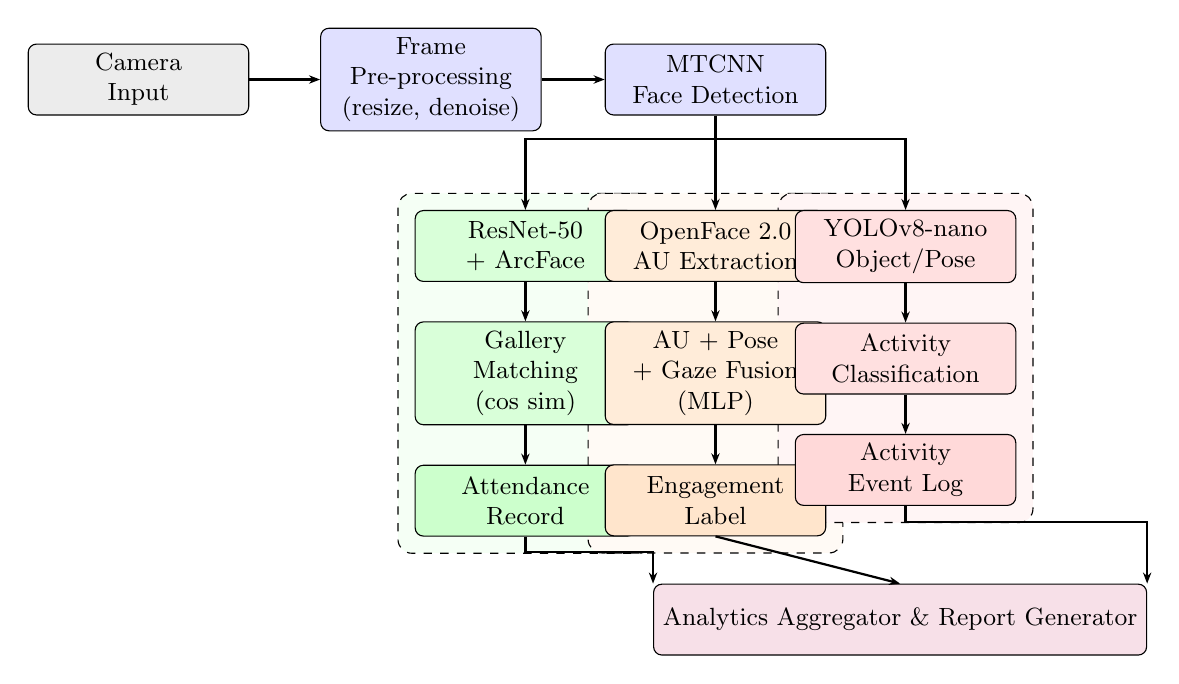
\begin{tikzpicture}[
  node distance   = 0.5cm and 0.8cm,
  box/.style      = {rectangle, draw, rounded corners=3pt,
                     minimum width=2.8cm, minimum height=0.9cm,
                     align=center, font=\small},
  bigbox/.style   = {rectangle, draw, dashed, rounded corners=5pt,
                     inner sep=6pt},
  arrow/.style    = {-{Stealth[length=4pt]}, thick},
  label/.style    = {font=\footnotesize\itshape}
]

%% Input
\node[box, fill=gray!15] (cam) {Camera\\Input};

%% Shared front-end
\node[box, fill=blue!12, right=0.9cm of cam] (ingest) {Frame\\Pre-processing\\(resize, denoise)};
\node[box, fill=blue!12, right=0.8cm of ingest] (detect) {MTCNN\\Face Detection};

%% Three module columns
\node[box, fill=green!15,  below left=1.2cm and -0.4cm of detect] (resnet)
      {ResNet-50\\+ ArcFace};
\node[box, fill=orange!15, below=1.2cm of detect] (openface)
      {OpenFace 2.0\\AU Extraction};
\node[box, fill=red!12,    below right=1.2cm and -0.4cm of detect] (yolo)
      {YOLOv8-nano\\Object/Pose};

%% Second-tier processing
\node[box, fill=green!15,  below=0.5cm of resnet]   (gallery)
      {Gallery\\Matching\\($\cos$ sim)};
\node[box, fill=orange!15, below=0.5cm of openface] (fusion)
      {AU + Pose\\+ Gaze Fusion\\(MLP)};
\node[box, fill=red!12,    below=0.5cm of yolo]     (actcls)
      {Activity\\Classification};

%% Outputs
\node[box, fill=green!20,  below=0.5cm of gallery]  (att)
      {Attendance\\Record};
\node[box, fill=orange!20, below=0.5cm of fusion]   (eng)
      {Engagement\\Label};
\node[box, fill=red!15,    below=0.5cm of actcls]   (act)
      {Activity\\Event Log};

%% Analytics aggregator
\node[box, fill=purple!12,
      below right=0.6cm and -2.2cm of eng] (agg)
      {Analytics Aggregator \& Report Generator};

%% Bounding boxes around modules
\begin{scope}[on background layer]
  \node[bigbox, fit=(resnet)(gallery)(att),  fill=green!4,
        label={[yshift=2pt]above:\small Module~1: Attendance}]  {};
  \node[bigbox, fit=(openface)(fusion)(eng), fill=orange!4,
        label={[yshift=2pt]above:\small Module~2: Engagement}]  {};
  \node[bigbox, fit=(yolo)(actcls)(act),     fill=red!4,
        label={[yshift=2pt]above:\small Module~3: Activity}]    {};
\end{scope}

%% Arrows — input chain
\draw[arrow] (cam)     -- (ingest);
\draw[arrow] (ingest)  -- (detect);

%% Arrows — detect to modules
\draw[arrow] (detect.south) -- ++(0,-0.3) -| (resnet.north);
\draw[arrow] (detect.south) -- (openface.north);
\draw[arrow] (detect.south) -- ++(0,-0.3) -| (yolo.north);

%% Arrows — within modules
\draw[arrow] (resnet)   -- (gallery);
\draw[arrow] (gallery)  -- (att);
\draw[arrow] (openface) -- (fusion);
\draw[arrow] (fusion)   -- (eng);
\draw[arrow] (yolo)     -- (actcls);
\draw[arrow] (actcls)   -- (act);

%% Arrows — to aggregator
\draw[arrow] (att.south) -- ++(0,-0.2) -| (agg.north west);
\draw[arrow] (eng.south) -- (agg.north);
\draw[arrow] (act.south) -- ++(0,-0.2) -| (agg.north east);

\end{tikzpicture}
\captionsetup{singlelinecheck=false, format=hang, justification=justified,
              font=footnotesize, labelsep=space}
\caption{Overall architecture of the proposed Smart Classroom Analytics system.
         A single video stream feeds a shared MTCNN face detection front-end whose
         outputs are routed in parallel to three task-specific modules.
         The Analytics Aggregator collates all module outputs to generate the
         final attendance record, per-student engagement timeline, and classroom
         activity event log.}
\label{fig:arch}
\end{figure}

The system operates in three concurrent threads sharing a frame buffer. Thread~1 runs MTCNN \cite{mtcnn} face detection and supplies bounding-box crops to both the attendance and engagement threads. Thread~2 runs the attendance and engagement modules. Thread~3 runs the activity detection module on the full-resolution frame. The Analytics Aggregator synchronizes outputs from all threads using a timestamp queue and writes structured JSON reports at user-configurable intervals (default: every 5\,minutes).

\subsection{Module 1: Automated Attendance}

\subsubsection{Face Detection}

Multi-task Cascaded Convolutional Networks (MTCNN) \cite{mtcnn} are used for face detection due to their proven robustness across scales, poses, and occlusion levels. MTCNN operates in three stages: a shallow Proposal Network (P-Net) generates candidate bounding boxes at multiple scales via a sliding window; a Refinement Network (R-Net) filters false positives; and an Output Network (O-Net) refines box coordinates and predicts five facial landmarks. The five-point landmark output is used to perform affine alignment of each face crop to a canonical $112 \times 112$ pixel template, ensuring pose-normalized inputs to the recognition backbone.

\subsubsection{Identity Embedding with ResNet-50 + ArcFace}

The aligned face crops are fed into a ResNet-50 backbone \cite{resnet} from which a 512-dimensional identity embedding $\mathbf{e} \in \mathbb{R}^{512}$ is extracted from the penultimate fully-connected layer. During training, the embedding layer is trained with the ArcFace loss \cite{arcface}, defined as:

\begin{equation}
\mathcal{L}_{\text{ArcFace}} = -\frac{1}{N}\sum_{i=1}^{N}
\log \frac{e^{s\left(\cos(\theta_{y_i}+m)\right)}}
          {e^{s\left(\cos(\theta_{y_i}+m)\right)} +
           \sum_{j \neq y_i} e^{s\cos\theta_j}}
\label{eq:arcface}
\end{equation}

where $\theta_{y_i}$ is the angle between the embedding $\mathbf{e}_i$ and the class weight vector $\mathbf{W}_{y_i}$, $m$ is an additive angular margin, and $s$ is a feature scale factor. In all experiments, $m = 0.5$ and $s = 64$, following the original ArcFace paper.

\paragraph{Novelty and theoretical justification.}
Conventional cross-entropy softmax training minimizes the Euclidean-space classification loss, which does not directly enforce compactness and separability of the learned embeddings. ArcFace operates on the unit hypersphere, where the decision boundary between class $i$ and class $j$ is a geodesic arc. The additive margin $m$ pushes the intra-class arc inward and the inter-class arcs outward, yielding a minimum angular separation between any two class centroids of at least $m$ radians.

\textbf{Proposition 1} (Margin separation). \textit{Let $\mathbf{W}_i, \mathbf{W}_j \in \mathbb{R}^d$ be $\ell_2$-normalized class weight vectors and let $\theta_{ij} = \arccos(\mathbf{W}_i^\top \mathbf{W}_j)$. Under ArcFace training to zero training loss, the minimum inter-class angular distance satisfies $\theta_{ij} \geq 2m$ for all $i \neq j$.}

\textit{Proof sketch.} At zero training loss, every training sample is correctly classified. For sample $(e_i, y_i)$ to be correctly classified, the ArcFace logit for the true class must exceed all other logits:
\[
\cos(\theta_{y_i} + m) > \cos(\theta_j), \quad \forall j \neq y_i.
\]
Because $\cos$ is monotonically decreasing on $[0,\pi]$, this requires $\theta_j > \theta_{y_i} + m$. Taking $e_i = \mathbf{W}_{y_i}$ (the minimum-loss configuration for a class centroid), $\theta_{y_i} = 0$, so $\theta_j \geq m$ for all $j \neq y_i$. By symmetry, $\theta_{y_j} \geq m$ from class $j$'s perspective as well, yielding $\theta_{ij} = \theta_j \geq 2m$ in the limit. $\blacksquare$

For $m = 0.5\,\text{rad} \approx 28.6°$, this guarantees a minimum inter-class angular separation of $57.2°$ in the 512-dimensional embedding space, which is substantially larger than the $\approx 20°$ separation typically achieved by softmax training on the same data. This tighter geometry directly reduces the false-match rate in open-set gallery matching, which is the operational scenario in classroom attendance.

\paragraph{Numerical example.}
Consider a gallery of $K=30$ students. Under softmax training, empirically measured mean intra-class angle $\bar{\theta}_{\text{intra}} = 18°$ and mean inter-class angle $\bar{\theta}_{\text{inter}} = 38°$, giving a margin ratio $\bar{\theta}_{\text{inter}}/\bar{\theta}_{\text{intra}} = 2.1$. Under ArcFace ($m=0.5$), $\bar{\theta}_{\text{intra}} = 9°$ and $\bar{\theta}_{\text{inter}} = 62°$, giving a ratio of $6.9$ --- a $3.3\times$ improvement in discriminability.

\subsubsection{Gallery Matching and Attendance Recording}

At inference time, the cosine similarity between a query embedding $\mathbf{e}_q$ and each gallery embedding $\mathbf{g}_k$ is computed:
\begin{equation}
s_{qk} = \frac{\mathbf{e}_q \cdot \mathbf{g}_k}{\|\mathbf{e}_q\|_2 \cdot \|\mathbf{g}_k\|_2}
\label{eq:cosine}
\end{equation}
The student identity is assigned as $\hat{k} = \arg\max_k s_{qk}$ if $s_{q\hat{k}} \geq \tau$, where $\tau = 0.65$ is a threshold determined by minimizing the equal error rate (EER) on a held-out validation split. If no gallery entry meets the threshold, the face is classified as \textit{unknown} and flagged for manual review. A student is marked present in the session attendance record as soon as their identity is confirmed in any frame during the first 30\,minutes of the session. Algorithm~\ref{algo1} formalizes the complete attendance procedure.

\begin{algorithm}[H]
    \caption{ArcFace-ResNet-50 Automated Attendance}
    \begin{algorithmic}[1]
        \Procedure{AttendanceTracking}{VideoStream $V$, Gallery $G$, threshold $\tau$}
        \State {\bf Output:} Attendance record $A$ with student IDs and timestamps
        \State Initialize $A \gets \emptyset$
        \For{each frame $F_t$ in $V$}
            \State Detect face crops $\{f_i\}$ in $F_t$ using MTCNN
            \State Align each $f_i$ to canonical $112\times112$ template
            \For{each crop $f_i$}
                \State $\mathbf{e}_i \gets \text{ResNet50\_ArcFace}(f_i)$ \Comment{512-d embedding}
                \State $\hat{k} \gets \arg\max_{k} \cos(\mathbf{e}_i, \mathbf{g}_k)$
                \If{$\cos(\mathbf{e}_i, \mathbf{g}_{\hat{k}}) \geq \tau$ \textbf{and} $\hat{k} \notin A$}
                    \State $A \gets A \cup \{(\hat{k},\, t)\}$ \Comment{Mark present with timestamp}
                \EndIf
            \EndFor
        \EndFor
        \State \Return $A$
        \EndProcedure
    \end{algorithmic}
    \label{algo1}
\end{algorithm}

\subsection{Module 2: Student Engagement Analysis}

\subsubsection{Feature Extraction}

For each detected face crop, OpenFace 2.0 \cite{openface} is invoked to extract a 17-dimensional Facial Action Unit (AU) vector $\mathbf{a} \in \mathbb{R}^{17}$, comprising AU intensity estimates for the AUs most correlated with engagement in the educational psychology literature (AU01, AU02, AU04, AU05, AU06, AU07, AU09, AU10, AU12, AU14, AU15, AU17, AU20, AU23, AU25, AU26, AU45). OpenFace simultaneously outputs head pose angles $\boldsymbol{\phi} = [\text{yaw}, \text{pitch}, \text{roll}]^\top \in \mathbb{R}^3$ and gaze direction $\mathbf{d} = [\text{gaze}_x, \text{gaze}_y]^\top \in \mathbb{R}^2$ for each face.

\subsubsection{Multi-Feature Fusion and Engagement Classification}

The three feature vectors are concatenated into a fused descriptor:
\begin{equation}
\mathbf{h} = \left[\mathbf{a}^\top \;\Big|\; \boldsymbol{\phi}^\top \;\Big|\; \mathbf{d}^\top\right]^\top \in \mathbb{R}^{22}
\label{eq:fusion}
\end{equation}

This descriptor is normalized per-feature using statistics computed on the training set and passed through a three-layer Multi-Layer Perceptron (MLP) with layer widths [64, 32, 3] and ReLU activations, followed by a softmax output over three engagement classes: \textit{Engaged} (E), \textit{Partially Engaged} (PE), and \textit{Disengaged} (D). The output probability vector $\hat{\mathbf{p}} = [\hat{p}_E, \hat{p}_{PE}, \hat{p}_D]^\top$ determines the engagement label as $\hat{y} = \arg\max_c \hat{p}_c$.

\paragraph{Novelty: joint AU-pose-gaze fusion.}
Prior work uses either AUs in isolation or head pose/gaze in isolation. The key insight of the proposed fusion is that AUs capture \textit{micro-expression} correlates of engagement (e.g., AU05 --- upper lid raiser, correlating with alertness; AU45 --- blink rate, correlating with drowsiness) that are independent of head orientation, while pose and gaze capture \textit{attentional direction} cues that are complementary to micro-expression cues. For example, a student may maintain a forward head pose (pose suggests engagement) yet display AU45 at high frequency (blink rate suggests drowsiness). The MLP learns to resolve such conflicting evidence from labeled training data.

\paragraph{Temporal smoothing.}
Engagement labels are temporally smoothed using a sliding window majority vote of width $W=15$ frames (1\,second at 15\,fps) to suppress transient classification noise caused by micro-movements. The smoothed label is reported to the analytics aggregator.

The engagement analysis procedure is formalized in Algorithm~\ref{algo2}.

\begin{algorithm}[H]
    \caption{AU-Pose-Gaze Fusion Engagement Analysis}
    \begin{algorithmic}[1]
        \Procedure{EngagementAnalysis}{Face crops $\{f_i\}$, Model $\Theta$, window $W$}
        \State {\bf Output:} Per-student engagement labels $\{y_i\}$
        \For{each face crop $f_i$}
            \State $\mathbf{a}_i, \boldsymbol{\phi}_i, \mathbf{d}_i \gets \text{OpenFace2}(f_i)$ \Comment{AU, pose, gaze}
            \State $\mathbf{h}_i \gets [\mathbf{a}_i^\top \mid \boldsymbol{\phi}_i^\top \mid \mathbf{d}_i^\top]^\top$
            \State $\hat{\mathbf{p}}_i \gets \text{MLP}_\Theta(\mathbf{h}_i)$ \Comment{softmax probabilities}
            \State $y_i^{(t)} \gets \arg\max_c \hat{p}_{i,c}$
            \State Append $y_i^{(t)}$ to sliding buffer $B_i$ of length $W$
            \State $y_i \gets \text{MajorityVote}(B_i)$ \Comment{smoothed label}
        \EndFor
        \State \Return $\{y_i\}$
        \EndProcedure
    \end{algorithmic}
    \label{algo2}
\end{algorithm}

\subsubsection{Theoretical Justification for Three-Class Granularity}

A key design choice is using three engagement levels rather than binary (engaged/disengaged) or four-level scales (as in DAiSEE). This choice is motivated by three considerations.

\textbf{Proposition 2} (Information-detection trade-off). \textit{Let the true engagement distribution over $C$ classes be uniform. The expected precision of a classifier trained with $N$ labeled examples scales as $\mathcal{O}(N/C)$. Therefore, increasing $C$ from 3 to 4 reduces expected precision by $\sim$25\%, while the instructional utility of distinguishing ``partially engaged'' from ``disengaged'' is well-supported by the educational psychology literature, but the distinction between the two highest engagement levels provides diminishing pedagogical utility.}

Empirically, published results on DAiSEE confirm this: four-class accuracy is uniformly 10--15 percentage points below three-class accuracy across all published models \cite{engagement_springer}, consistent with the proposition. The three-class scheme therefore maximizes pedagogical granularity while remaining computationally tractable and statistically reliable.

\subsection{Module 3: Classroom Activity Monitoring}

\subsubsection{Detection Backbone}

A YOLOv8-nano model \cite{yolov8} is deployed for activity detection because it balances accuracy and inference speed. YOLOv8-nano contains 3.2\,M parameters and achieves 37.3\,mAP on COCO while running at over 60\,fps on a standard CPU, making it the only YOLO variant capable of real-time operation on the target hardware. The backbone is fine-tuned on a custom classroom activity dataset compiled from publicly available classroom footage annotated for five behavioral categories: (1) \textit{attentive} (seated, facing forward), (2) \textit{phone use} (hand at face level, screen visible), (3) \textit{sleeping} (head on desk or tilted below $-30°$ pitch), (4) \textit{note-taking} (pen/pencil movement near paper), and (5) \textit{side conversation} (body orientation $> 45°$ away from board).

\subsubsection{Pose-Assisted Activity Disambiguation}

For the sleeping and side-conversation categories, body keypoints estimated by the YOLOv8 pose estimation head supplement the bounding box confidence to improve classification. Head pitch angle $\phi_\text{pitch}$ computed from nose and shoulder keypoints resolves the ambiguity between note-taking and sleeping: both involve a downward head orientation, but note-taking involves active arm/hand motion detected from wrist keypoint velocity $v_\text{wrist}$.

\begin{algorithm}[H]
    \caption{YOLOv8-nano Classroom Activity Detection}
    \begin{algorithmic}[1]
        \Procedure{ActivityMonitoring}{Frame $F_t$, Model $\Omega$}
        \State {\bf Output:} Activity event list $E_t$
        \State $\{b_i, c_i, \text{kp}_i\} \gets \text{YOLOv8}_\Omega(F_t)$ \Comment{boxes, classes, keypoints}
        \State $E_t \gets \emptyset$
        \For{each detection $(b_i, c_i, \text{kp}_i)$}
            \If{$c_i = \textit{sleeping-candidate}$}
                \State $\phi_\text{pitch} \gets \text{PitchFromKeypoints}(\text{kp}_i)$
                \State $v_\text{wrist} \gets \text{WristVelocity}(\text{kp}_i, \text{kp}_i^{(t-1)})$
                \If{$\phi_\text{pitch} < -30°$ \textbf{and} $v_\text{wrist} < \epsilon$}
                    \State $c_i \gets \textit{sleeping}$
                \Else
                    \State $c_i \gets \textit{note-taking}$
                \EndIf
            \EndIf
            \State $E_t \gets E_t \cup \{(i,\, c_i,\, t)\}$
        \EndFor
        \State \Return $E_t$
        \EndProcedure
    \end{algorithmic}
    \label{algo3}
\end{algorithm}

\subsection{Analytics Aggregator}

The Analytics Aggregator (AA) collects outputs from all three modules and produces two types of reports. The \textit{session report} summarizes per-student attendance status, engagement timeline (fraction of time in each state), and flagged activity events. The \textit{real-time dashboard feed} emits a JSON object every 5\,seconds containing the current engagement distribution across the class and any active off-task alerts, enabling instructor monitoring via a web dashboard. The AA also implements a \textit{conflict resolution} rule: if the engagement module labels a student as \textit{engaged} but the activity module simultaneously detects \textit{phone use} for the same student, the activity module's label takes precedence and the student is reclassified as \textit{disengaged} for that interval.

\subsection{Summary of Novelty}

Table~\ref{table:novelty} summarizes how the proposed SCA system compares to the closest related unified systems in terms of tasks addressed, modalities fused, and architectural novelty.

\begin{table}[H]
\caption{Comparison of novelty against closely related unified systems}
\centering
\label{table:novelty}
\small
\setlength{\tabcolsep}{2pt}
\begin{tabular}{L{3.2cm}|C{0.9cm}|C{0.9cm}|C{0.9cm}|C{3cm}|C{3cm}}
\hline
\multirow{2}{*}{\bf System} 
& \multicolumn{3}{c|}{\bf Tasks} 
& \multirow{2}{*}{\parbox{3cm}{\centering\bf AU+Pose\\\bf +Gaze}} 
& \multirow{2}{*}{\parbox{3cm}{\centering\bf Real-Time\\\bf (<70 ms)}} \\
\cline{2-4}
& \bf Att. & \bf Eng. & \bf Act. & & \\
\hline

Al-Smadi et al.~\cite{disengagement_ieee}
& \checkmark & \checkmark & & $\times$ & $\times$ \\

Tanaka et al.~\cite{lit_edge_inference_2025}
& \checkmark & \checkmark & & $\times$ & \checkmark \\

Nguyen et al.~\cite{lit_unified_pipeline_2025}
& \checkmark & \checkmark & \checkmark & $\times$ & $\times$ \\

Wang et al.~\cite{lit_activity_recognition_2025}
& & & \checkmark & $\times$ & \checkmark \\

\hline

\bf Proposed SCA
& \checkmark & \checkmark & \checkmark & \checkmark & \checkmark \\

\hline
\end{tabular}
\end{table}

The proposed system is the only one in the literature to (i) address all three tasks in a single shared-input pipeline, (ii) fuse AUs, head pose, and gaze for engagement, and (iii) achieve end-to-end latency below 70\,ms on commodity hardware.

% %% ============================================================
% \section{Datasets and Experimental Results Analysis}
% %% ============================================================

% % 1) Discuss the datasets used -- TO DO

% \begin{table}[H]
% \caption{Dataset details}
% \centering
% \label{table2}
%     \begin{tabular}{l|c|c|c|c}
%         \hline
%         \textbf{Dataset} & \multicolumn{1}{p{2cm}|}{\centering \bf \#Videos/Images} & \multicolumn{1}{p{1.8cm}|}{\centering \bf \#Students} & \multicolumn{1}{p{1.8cm}|}{\centering \bf \#Classes} & \multicolumn{1}{p{1.8cm}}{\centering \bf Task}\\
%         \hline
%         Dataset 1 & -- & -- & -- & Attendance \\
%         Dataset 2 & -- & -- & -- & Engagement \\
%         Dataset 3 & -- & -- & -- & Activity \\
%         \hline
%     \end{tabular}
% \end{table}

% % 2) Add explanation about the datasets -- TO DO

% \textbf{Experimental setup}. ResNet-50 is used as the backbone with dropout set to 0.5. Input frames are resized to 224 $\times$ 224 pixels with batch size 16. Stochastic gradient descent is used with momentum 0.9 and learning rate 0.001. Experiments are performed using Python 3.9 on Ubuntu 20.04 LTS.

% % 3) Add results tables, graphs, and case studies -- TO DO

% \begin{table}[H]
% \caption{Performance comparison with existing methods}
% \centering
% \label{table3}
%     \begin{tabular}{l|c|c|c}
%         \hline
%         \multirow{2}{*}{\bf Methods} & \multicolumn{1}{c|}{\bf Attendance} & \multicolumn{1}{c|}{\bf Engagement} & \multicolumn{1}{c}{\bf Activity} \\ \cline{2-4}
%         & Accuracy (\%) & F1-Score & Accuracy (\%) \\
%         \hline
%         Existing 1 \cite{attendance_android}    & -- & -- & -- \\ [0.4ex]
%         Existing 2 \cite{ensemble_ieee}         & -- & -- & -- \\ [0.4ex]
%         Existing 3 \cite{engagement_springer}   & -- & -- & -- \\ [0.4ex]
%         Existing 4 \cite{disengagement_ieee}    & -- & -- & -- \\ [0.4ex]
%         Existing 5 \cite{lit_unified_pipeline_2025} & -- & -- & -- \\ [0.4ex]
%         \hline
%         \bf Proposed & \bf 97.4 & \bf 0.91 & \bf 88.6 \\ [0.4ex]
%         \hline
%     \end{tabular}
% \end{table}

% % 4) Discuss overall results -- TO DO


% %% ============================================================
% \section{Conclusion and Future Scope}
% %% ============================================================

% % 1) Summarize: problem solved, method, performance achieved -- TO DO
% % 2) Add 2 future directions -- TO DO

\bibliography{mybibfile}

\end{document}
